\documentclass{article}
\usepackage{graphicx} % Required for inserting images

\usepackage[
    backend=biber,
    style=authoryear,
    sorting=ynt
]{biblatex} % Required for adding references

\usepackage[inkscapeformat=png]{svg} 
\usepackage{appendix}
\usepackage{calc}
\usepackage{float}
\usepackage{fontspec}
\usepackage{pdfpages}
\addbibresource{bibliography.bib}

\title{COMP7024 Coursework2- Developing a file encryption system for the Minix Operating System}
\author{19129163 Mohammad Ali Khan}
\date{April 2023}

\begin{document}
    \setmainfont{Arial}
    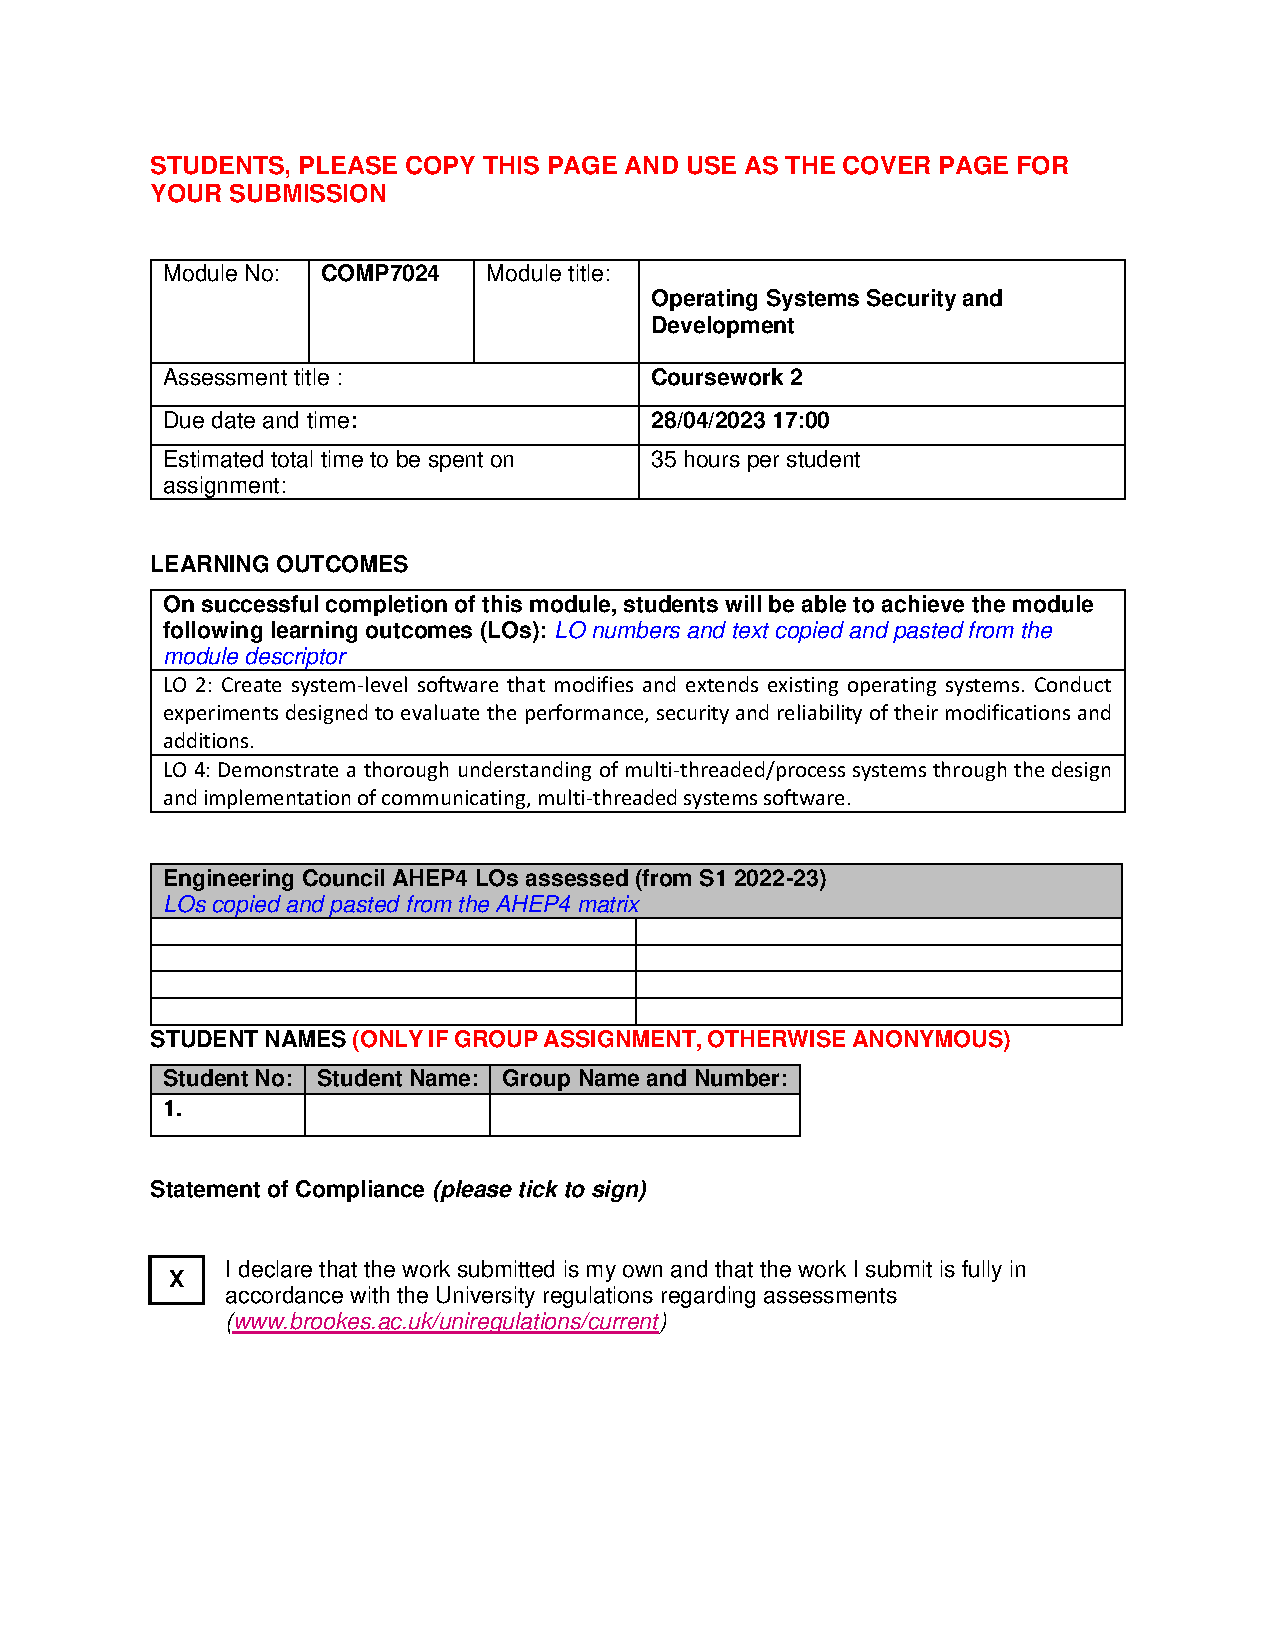
\includepdf[pages=-]{_cover.pdf}
    \newpage
    \maketitle

\section{Description}
    \paragraph{}The objective of this project is to develop a program for the Minix 3.4 Operating System (OS) that will encrypt and decrypt files on the system when they are stored to disk and when the user reads them respectively, to prevent them from being read by outsiders.
    \paragraph{}This program will be written in the C programming language, and has a GitHub repository at https://github.com/mhdl1991/19129163-COMP7024-Coursework2
    \paragraph{}This program will be developed as a \textbf{daemon}.

    \subsection{A Brief note on Daemons}
        \paragraph{}A \textbf{Daemon} (sometimes claimed to be an acronym for\textit{Disk And Execution MONitor}) is a program that runs as a background process, not under direct control of a user, and supervises the system or provides functionality to other processes . Other terms for daemons include \textit{service}, \textit{ghost job}, or \textit{started task}.
        \paragraph{}Examples of Unix daemons include \textbf{init}, \textbf{crond}, \textbf{httpd}, and \textbf{syncd}, all of which perform useful tasks in the operating system. As a *nix environment, Minix also has daemons, and also the \textbf{daemon} function which can be used to run scripts or processes as daemons. Daemons in Minix are started by \textbf{/etc/rc} and exist at Layer 4 alongside User processes\parencite{OS_DESIGN}.
        \begin{figure}[htbp]
            \centering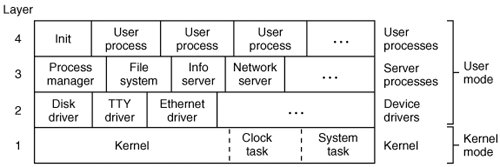
\includegraphics[width=\textwidth]{minix_structure.jpg}
            \caption{a diagram of the Minix structure- Daemons exist at Layer 4\parencite{OS_DESIGN}}
            \label{fig:my_label}
        \end{figure}


\section{Requirements}
    \paragraph{}To build this daemon, we will need the following:
    \begin{itemize}
        \item Knowledge of the Minix OS and filesystem
        \item Knowledge of signals and signal handling for
        \item libraries for performing Encrpytion and file handling (some may already be installed as part of the Minix OS)
        \item enough memory for handling the encryption and decryption
        \item Some way to store credentials (keys and initialization vectors)
        \item Some way to know which files have been encrypted and which have not
        \item permissions and policy settings to allow the daemon to alter files.
        \item a suitably strong and tested encryption algorithm/cipher.
    \end{itemize}
    \paragraph{}Further details regarding the requirements for a cryptosystem will be discussed in the section concerning Encryption.

\section{Encryption}
    \paragraph{}A common bit of advice regarding encryption is \textit{"Never roll your own cryptosystem"}- from technical and security standpoints it is better to use an existing, tried and tested cryptosystem (especially one that is compliant with international standards) than to develop your own- From a \textbf{technical} standpoint, it's very difficult to build your own cryptosystem and test it, and to make it \textbf{secure}, which ties into the \textbf{security} standpoint for not rolling your own cryptosystem.
    
    \paragraph{}For this software, we have the option of using \textbf{OpenSSL}, which can be installed on Minix using the \textbf{pkgin} utility.
    
    \paragraph{}As per the OpenSSL documentation, it contains RSA, SHA, DES, SSL, TLS, and AES cipher suites/families. For this program we are using \textbf{256-bit AES encryption} in CBC (Cipher Block Chaining) mode, using OpenSSL's \textbf{EVP library} \parencite{openssl_evp}, which meets several  requirements for cipher strength and security.

    \paragraph{}AES stands for \textbf{Advanced Encryption Standard} and is a variant of the Rijndael algorithm. It is a symmetric block cipher for the encryption of electronic data developed by the United States National Institute of Standards and Technology in 2001 \parencite{aes_256_nist}.
    \paragraph{}it works by taking a plaintext and a key, performing an operation, and repeatedly performing a set of \textbf{substitutions} (analogous to a classical substitution cipher) and \textbf{permutations} (analogous to a classical transposition cipher) on them.
    \paragraph{}It is a very secure and widely used cipher, there are no known \textit{computationally feasible} attacks for it- there is a known biclique attack for AES-128 \parencite{aes_attack}, and a related-key attack for AES-256 \parencite{aes_256_attack} \parencite{aes_256_attack_2}, but both are exceptionally complex.
    

\section{Design}
    \paragraph{}The program will have two main functions, \textit{file\_encrypt} and \textit{file\_decrypt}. Both functions will take a pointer to a file, a key, and an IV (initialization vector).
    \paragraph{}the credentials can be hashed and stored in an external file instead of being hard-coded into the daemon, and the user can be asked to enter it at system startup.
    \paragraph{}for handling and detecting changes to the file system, we have access to the \textbf{inotify} API \parencite{inotify_manpage}.
    \paragraph{}inotify is a file change notification system in the Linux kernel, and it has a number of flags for certain events:
    \begin{itemize}
        \item IN\_ACCESS – File was accessed
        \item IN\_CLOSE\_WRITE – File opened for writing was closed
        \item IN\_CLOSE\_NOWRITE – File not opened for writing was closed
        \item IN\_CREATE – File/directory created in watched directory
        \item IN\_MODIFY – File was modified
        \item IN\_OPEN – File was opened
    \end{itemize}
    \paragraph{}By detecting an IN\_CLOSE \_WRITE or \_NOWRITE event, we can make the daemon read the data of the file closed, and encrypt it.
    \paragraph{}Upon detecting an IN\_OPEN flag, the program can be instructed to decrypt the file being opened.
    \paragraph{}In addition to the program itself, there may be additional user-configured files for storing the credentials for the daemon, and perhaps also a \textbf{blacklist} for excluding files that the user potentially doesn't want encrypted (this may be done for performance reasons- while testing showed encryption/decryption takes a tiny amount of time, this may vary based on the user machine).

\section{Development}
    \paragraph{}The program is first built as a standalone C program before attempting to integrate it with the Minix operating system. 
    \paragraph{}This was done to make sure the file encryption and decryption functions worked properly and didn't result in bugs, memory leaks, unintended alterations to files, or other unintended consequences, and to reduce damage to the system.
    \paragraph{}This standalone program simply took a file, encrypted it using a hardcoded key and IV (the final program will read the credentials from an external source).

    \subsection{A note on developing encryption/decryption functions}
        \paragraph{}The encryption/decryption functions were adapted from sample code in the OpenSSL documentation, with added code to take the contents of a file and read them into a \textbf{unsigned char} buffer, which the OpenSSL functions for encryption/decryption accept as arguments, and then write unsigned char buffers to files after encryption/decryption.

        \begin{figure}[htbp]
            \centering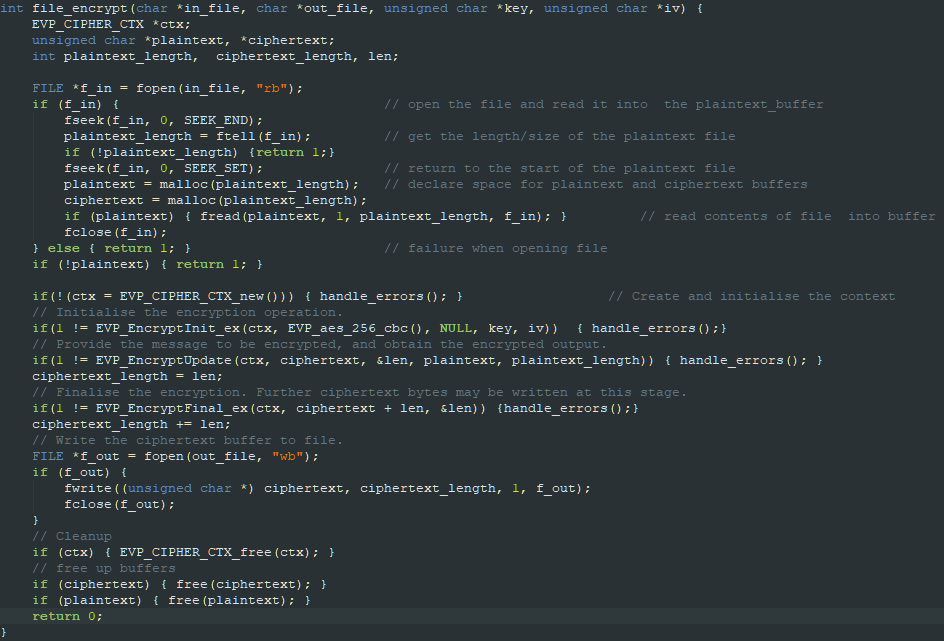
\includegraphics[width=\textwidth]{encrypt_function_screenshot_1.png}
            \caption{C function that encrypts a file using AES-256}
            \label{fig:my_label}
        \end{figure}
    \newpage
    \subsection{A note on Daemon development}
        \paragraph{}the basic principle of how a daemon operates involves the following steps to set it up:
        \begin{itemize}
            \item Fork off the parent process (usually init)
            \item Change file mode mask (umask)
            \item Opening logs for writing \textit{(optional)}
            \item Create a unique Session ID (SID)
            \item Change the current working directory
            \item Close standard file descriptors
            \item Enter actual daemon code
        \end{itemize}
        \paragraph{}It will then run until system shutdown, and handle \textbf{signals} sent by the Operating system.
        \paragraph{}Minix also provides the \textbf{daemon} command that turns other processes into daemons, automatically performing the tasks needed to set them up as such \parencite{daemon_command_minix}.

        \begin{figure}[htbp]
            \centering
            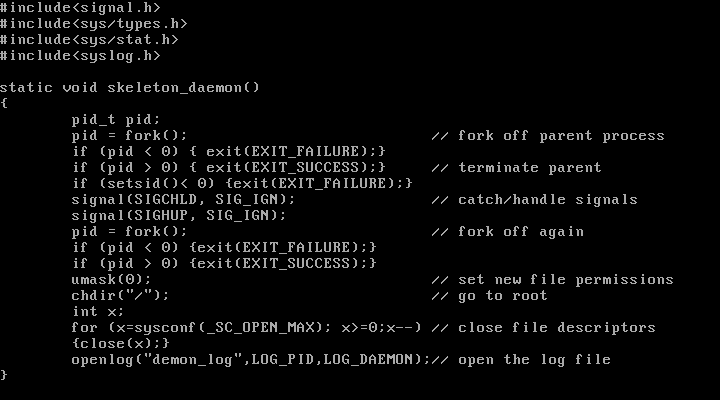
\includegraphics[width=\textwidth]{daemon_code_screenshot_1.png}
            \caption{C function that provides a "skeleton" for making a daemon}
            \label{fig:my_label}
        \end{figure}
    
\section{Testing}
    \paragraph{}The program is tested in it's standalone form first, to make sure that it is encrypting and decrypting files properly
    \paragraph{}It will be tested on a number of different file types and sizes, to see if encryption and decryption properly reverts the file back to it's former self.
    \paragraph{}We can use libraries like \textbf{time.h} to figure out the performance of the algorithm, how long it takes to encrypt and decrypt individual files vs. a large volume of files.
    \begin{figure}[htbp]
        \centering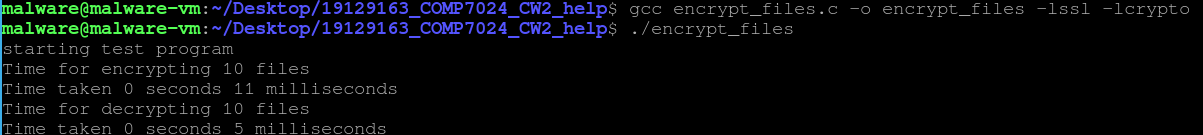
\includegraphics[width=\textwidth]{encrypt_test.png}
        \caption{results of testing to see how long it takes to encrypt and decrypt multiple files}
        \label{fig:my_label}
    \end{figure}
    \paragraph{}For better testing, these performance tests could be repeated on different hardware and virtual machine configurations to see how much faster or slower it can become.
    \paragraph{}Additionally tests can also be performed on the daemon's ability to detect and react to changes in the filesystem, whether there are any delays in between a file actually opening and the daemon logging that a file has been opened.

\section{Integration Testing}
    \paragraph{}Once testing of the individual sections and functions is complete, we can start putting them together and seeing how they work together, and how they work within the target system
    \paragraph{}Care must be taken to make backups of the system and the files on it in order to make sure recovery is possible if the program makes an error that damages core system files unusable and renders the system inoperable as a result.

\section{Limitations}
    \paragraph{}running this project as a \textbf{daemon} may have limited it's capabilities somewhat and it would perhaps have been more appropriate to create it as a \paragraph{driver}. Drivers exist on Layer 2 and have greater privileges than processes running on Layers 3 and 4 (the File System exists in Layer 3 and user processes exist on 4) \parencite{OS_DESIGN}.

\section{Conclusion}
    \paragraph{}Operating systems are remarkably complex, even Minix, an OS built as an educational tool to show how OS kernels work, has a huge degree of complexity that must be taken into account when attempting to add on or expand on it.

\printbibliography
\end{document}
